\section{Effect and Propagation of Systematic Uncertainties}
\label{sec:physics-lbnosc-syst}\label{sec:nu-osc-09}

%Content will include: 
%\begin{itemize}
%    \item Overview of the systematic uncertainties
%    \item Discussion of cancellations and constraints
%    \item Discussion of what has the largest impacts on sensitivities
%    \item Potential sources of bias
%\end{itemize}

%\subsubsection{Uncertainties \& Constraint Requirements from ND Analyses}
%Potential figures and tables include: 
%\begin{itemize}
%\item Error envelopes (vs energy) pre and post ND constraints (New plot)
%\item CafAna response functions examples 
%\item CafAna chisq vs paramater constraint examples 
%\item Table: Parameter constraints with pre/post fit $1\sigma$ uncertainties per %systematic (New)
%\item Covariance matrix 
%\item (Placeholder added) Example DUNE PRISM style prediction with representative cancellation of uncertainties.
%\item (Placeholder added) Missing proton energy fake data study bias demonstration and resolution.
%\end{itemize}

Systematic uncertainties can be broadly divided into three categories: flux, neutrino interactions, and detector effects. Flux uncertainties are described in Section~\ref{sec:nu-osc-05}. Neutrino cross section uncertainties are described in Section~\ref{sec:nu-osc-05}. Detector-related uncertainties are described in Section~\ref{sec:detSysts}. The remainder of this section will cover the ways in which uncertainties are constrained in the near-far oscillation fit, and the individual uncertainties with the largest impact on oscillation parameter sensitivities.

\subsection{Detector Systematic Uncertainties}
\label{sec:detSysts}

Detector efDetector effects impact the event selection efficiency as well as the reconstruction of quantities used in the oscillation fit, such as neutrino energy. The main sources of detector systematic uncertainties are limitations of calibration and modeling of particles in the detector. While neutrino interaction uncertainties can also affect reconstruction, this section is focused on effects that arise from the detectors.

The near LAr TPC detector uses a similar technology as the far detector, namely they are both liquid argon TPCs. However, important differences lead to uncertainties that do not fully correlate between the two detectors. First, the readout technology is different, as the near LAr TPC uses pixels as well as a different, modulear photon detector. Therefore, the charge response to particle types (e.g. muons and protons) will be different between near and far due to differences in electronics readout, noise, and local effects like alignment.  Second, the high-intensity environment of the ND complicates associating detatched energy deposits to events, a problem which does not exist in the FD. Third, the calibration programs will be very different. For example, the near detector has a high-statistics calibration sample of through-going, momentum-analyzed muons from neutrino interactions in the upstream rock, which does not exist for the FD. Conversely, the local electric field in the ND will be complicated by ion accumulation (space charge) as it has much less overburden than the FD. Finally, the reconstruction efficiency will be inherently different due to the relatively small size of the ND. Containment of charged hadrons will be significantly worse at the ND, especially for events with energetic hadronic showers or which vertex near the edges of the fiducial volume. Detector systematics in the gaseous TPC at the near site will be entirely uncorrelated to the far detector.

\subsubsection{Energy scale uncertainties}
\label{sec:EnergyScaleSysts}

Uncertainties on the overall energy response are implemented, as well as particle response uncertainties that are different for muons, charged hadrons, neutrons, and electromagnetic showers. Some are partially correlated between the near and far detectors, for example the muon energy in liquid argon. Others are treated as fully uncorrelated, for example the curvature-based MPT muon reconstruction. Observed neutron energy is treated as uncorrelated due to the anticipated challenges of associating neutrons. The full list of energy scale uncertainties is given as Table~\ref{tab:EscaleSysts}.

The scale of these uncertainties is derived from recent experiments, including calorimetric based approaches (NOvA, MINERvA) and liquid Argon TPCs (LArIAT, MicroBooNE, ArgoNEUT). On NOvA~\cite{NOvA:2018gge}, the muon (proton) energy scale achieved is $<1$\% (5\%). Uncertainties associated to the pion and proton re-interactions in the detector medium are expected to be controlled from ProtoDUNE and LArIAT data, as well as the combined analysis of low density (gaseous) and high density (LAr) near detectors. Uncertainties in the electric field also contribute to energy scale, and calibration is needed (with cosmics at ND, laser system at FD) to constrain the overall energy scale. The recombination model will continue to be validated by the suite of LAr experiments and is not expected to be an issue for nominal field provided minimal E-field distortions. 
Uncertainties in the electronics response is controlled with dedicated charge injection system and validated with intrinsic sources (Michel electrons, Ar(39)).
The response of the detector to neutrons is a source of active study and will couple strongly to detector technology. The validation of neutron interactions in LAr will continue to be characterized by dedicated measurements (CAPTAIN) and the LAR program (e.g. ArgoNEUT~\cite{PhysRevD.99.012002}).  However, the association of the identification of a neutron scatter or capture to the neutrons true energy has not been demonstrated, and significant reconstruction issues exist, so a large uncertainty (20\%) is assigned comparable to the observations made by MINERvA~\cite{Elkins:2019vmy} assuming they are attributed entirely to the detector model. Selection of photon candidates from $\pi^0$ is also a significant reconstruction challenge, but a recent measurement from MicrbooNE indicates this is possible and the $\pi^0$ invariant mass has an uncertainty of 5\%, although with some bias~\cite{Adams:2018sgn}.

\begin{dunetable}[Energy scale systematics]{c|ccc}{tab:EscaleSysts}
{Uncertainties applied to the energy response of various particles at the near and far detectors.}
    Systematic & Particle(s) & ND effect & FD effect \\ \toprowrule
    Muon LAr  & $\mu$ & 1\% (LAr contained) & 1\% \\
    Muon GAr ND & $\mu$ & 1\% & 0 \\
    Electron & $e$ & 2\% & 2\% \\
    Charged hadron Correlated & $p, \pi^{\pm}$ & 5\% & 5\% \\
    Charged hadron ND &  $p, \pi^{\pm}$ & 1\% & 0 \\
    Charged hadron FD &  $p, \pi^{\pm}$ & 0 & 1\% \\
    Neutron ND & $n$ & 20\% & 0 \\
    Neutron FD & $n$ & 0 & 20\% \\
    $\pi^{0}$ Correlated & $\pi^{0}$ & 5\% & 5\% \\
    $\pi^{0}$ ND & $\pi^{0}$ & 2\% & 0 \\
    $\pi^{0}$ FD & $\pi^{0}$ & 0 & 2\% \\
    \hline
\end{dunetable} 

\subsubsection{Reconstruction efficiency uncertainties}

Uncertainties are evaluated on the muon and hadron acceptance, as well as on the energy reconstruction. The detector acceptance for muons and hadrons is shown in Figure~\ref{fig:NDreco}. Inefficiency at very low lepton energy is due to events being misreconstructed as neutral current, which can also be seen in Figure~\ref{fig:recoEvcats}. For high energy, forward muons, the inefficiency is only due to events near the edge of the fiducial volume where the muon misses the MPT. At high transverse momentum, muons begin to exit the side of the LAr active volume, except when they happen to go along the 7m axis. The acceptance is sensitive to the modeling of muons in the detector. An uncertainty is estimated based on the change in the acceptance as a function of muon kinematics.

Inefficiency at high hadronic energy is due to the veto on more than 30 MeV deposited in the outer 30cm collar of the active volume. Rejected events are typically poorly reconstructed due to low containment, and the acceptance is expected to decrease at high hadronic energy. Similar to the muon reconstruction, this acceptance is sensitive to detector modeling, and an uncertainty is evaluated based on the change in the acceptance as a function of true hadronic energy.

\subsection{Systematic Uncertainty Constraints and Cancellations}

Flux and cross section uncertainties are constrained in the fit, especially by the near detector. Figure~\ref{fig:postfit_uncertainties} shows the level of constraint on each systematic parameter after the fit.

\begin{dunefigure}[Post-fit systematic uncertainties]{fig:postfit_uncertainties}
{PRELIMINARY, needs updating: The ratio of post-fit to pre-fit uncertainties for various systematic parameters. The shaded region is with a one-dimensional near detector fit to neutrino energy only, while the hatched region includes the full two-dimensional near detector spectra in neutrino energy and inelasticity.}
  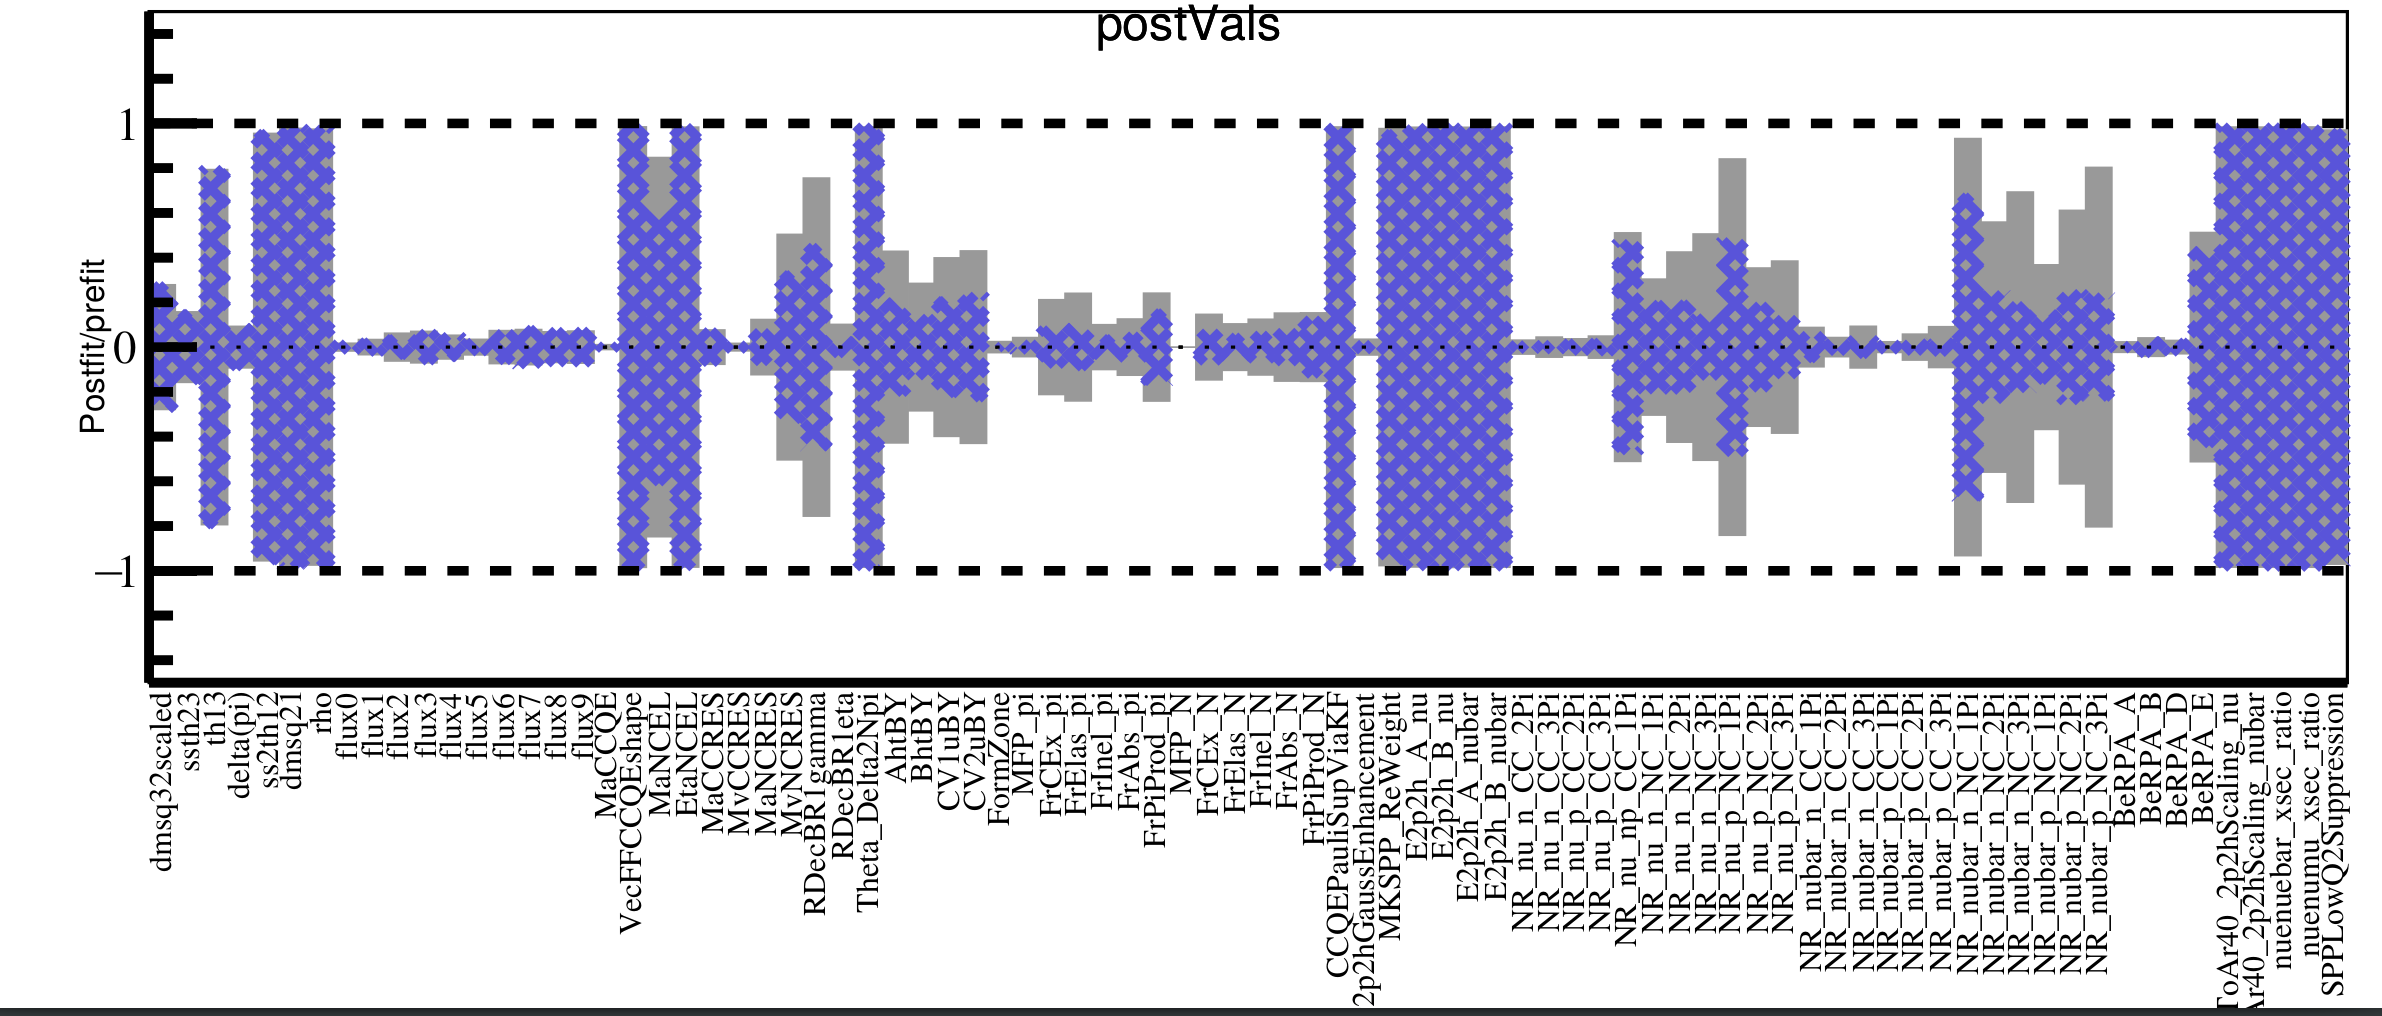
\includegraphics[width=0.9\textwidth]{graphics/postfit_errors.png}
\end{dunefigure}

\fixme{Analysis in progress}

%\fixme{Pre- and Post-fit error matrices}

\subsection{Largest Systematic Uncertainties}

Uncertainties do not fully cancel with the near detector constraint. In this section, the largest sources of systematic uncertainty are discussed. Also, the fit introduces anticorrelations between parameters, especially between the flux and cross sections.

\fixme{Analysis in progress}

\subsection{Avoiding bias}

\begin{figure}[h]
\centering
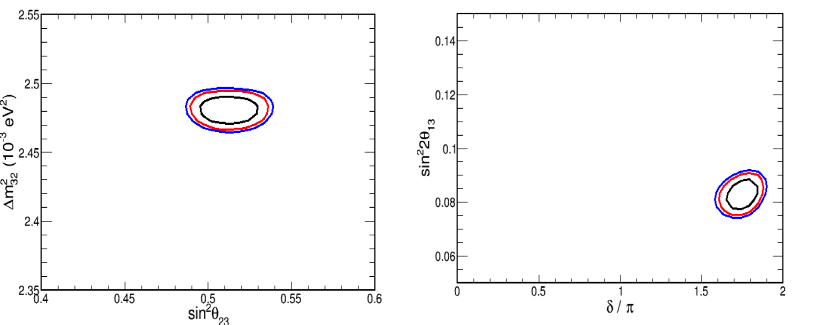
\includegraphics[angle=0,width=16cm,height=5.6cm]{protonEbias_fluxfloated.png}
\caption{Contours of fitting 20\% missing proton energy fake data for true oscillated parameters corresponding to  sin$^{2}\theta_{23}$=0.5, $\Delta$m$^{2}_{23}$=2.45x10$^{-3}$ eV$^{2}$, $\Delta$=1.5$\pi$ and sin$^{2}2\theta_{13}$=0.085. Nuisance parameters corresponding the flux allowed to float.
Left: sin$^{2}\theta_{23}$ vs. $\Delta$m$^{2}_{32}$ Right: $\delta$ vs. sin$^{2}2\theta_{13}$) planes with flux constraints.} \label{protonFDSbias}
\end{figure}
\fixme{Stars will be added to the plot to indicate the true values of the parameters}

Figure~\ref{protonFDSbias} shows how measurements of oscillation may be biased due to mis-modelling in the interaction model. This specific mock data, described in Section~\ref{sec:nu-osc-05}, is a plausible modification to the reconstructed-true energy association. Furthermore, the underlying cross section model issue is not visible with only the on-axis event sample, as shown in Fig~\ref{fig:protonFDS_spectra1}. However, off-axis samples show disagreement with the on-axis-only ND fit; off-axis samples may be used to diagnose and resolve underlying interaction mis-modelling~\ref{fig:protonFDS_spectra2}. %\fixme{Mike: please read and expand/adjust}


\begin{figure}[h]
\centering
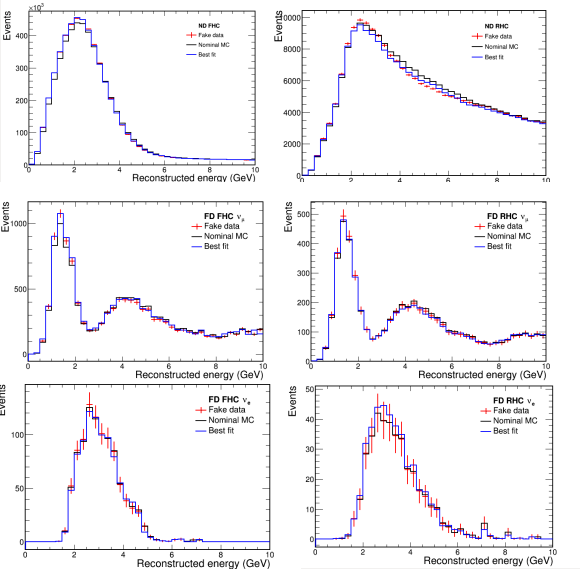
\includegraphics[angle=0,width=16cm,height=15.6cm]{protonFDS_spectra1.png}
\caption{20\% missing proton energy fake data fitting spectra for ND and FD FHC and RHC with flux constraints. The black spectra are nominal, the red are fake data and the blue are best fit.}
\label{fig:protonFDS_spectra1}
\end{figure}

\begin{figure}[h]
\centering
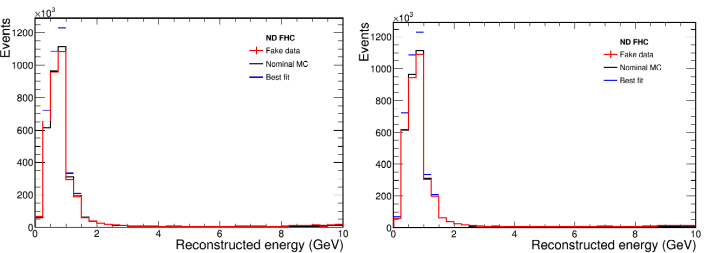
\includegraphics[angle=0,width=16cm,height=5.6cm]{protonFDS_spectra2.png}
\caption{With flux parameters, comparison of on-axis best fit(blue), 30 m off-axis nominal(black) and 30 m off-axis fake data(red) spectra. Left: FHC; Right: RHC. }
\label{fig:protonFDS_spectra2}
\end{figure}
%\fixme{The oscillated fake data spectra can be removed here to save space}